\documentclass{standalone}
\usepackage{tikz}

\begin{document}

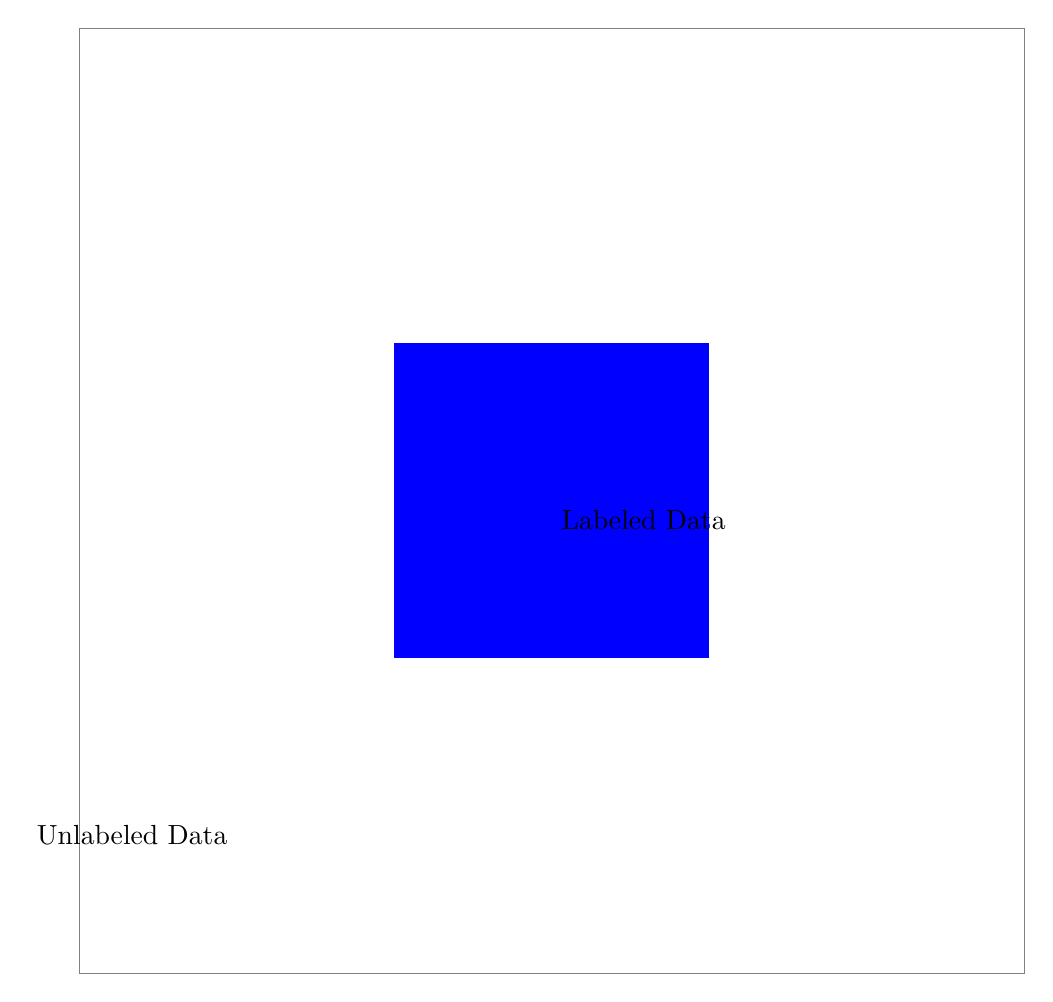
\begin{tikzpicture}[scale=2]
    % Draw the labeled (blue) area
    \fill[blue] (-1,-1) rectangle (1,1);
    
    % Draw the unlabeled (gray) area
    \draw[gray] (-3,-3) rectangle (3,3);
    
    % Add labels for clarity
    \node at (-2,-2) [below left] {Unlabeled Data};
    \node at (0,0) [below right] {Labeled Data};
\end{tikzpicture}

\end{document}